\section{Implementasi Fitur Utama}
\subsection{Upload dan Pratinjau PDF}
Pengguna dapat mengunggah file PDF yang akan disimpan pada \texttt{Vercel Blob}. File ini kemudian dimuat dan dipratinjau menggunakan \texttt{PDF.js}.
\begin{lstlisting}[language=TypeScript, caption={Chat dengan AI}]
'use client';

import { ChatHeader } from '@/components/chat-header';
import { useArtifactSelector } from '@/hooks/use-artifact';
import type { Vote } from '@/lib/db/schema';
import { fetcher, generateUUID } from '@/lib/utils';
import { useChat } from '@ai-sdk/react';
import type { Attachment, UIMessage } from 'ai';
import type { Session } from 'next-auth';
import { useRouter, useSearchParams } from 'next/navigation';
import { useEffect, useRef, useState } from 'react';
import useSWR, { useSWRConfig } from 'swr';
import { unstable_serialize } from 'swr/infinite';
import { Artifact } from './artifact';
import { Messages } from './messages';
import { MultimodalInput } from './multimodal-input';
import { getChatHistoryPaginationKey } from './sidebar-history';
import { toast } from './toast';
import type { VisibilityType } from './visibility-selector';

import dynamic from 'next/dynamic';
const PDFViewer = dynamic(() => import('../components/pdf-viewer'), {
  ssr: false,
});

import { Show } from './shared/show';
import { useBoolean } from '@/hooks/use-boolean';
import { useMediaQuery } from 'usehooks-ts';

export function Chat({
  id,
  initialMessages,
  selectedChatModel,
  selectedVisibilityType,
  isReadonly,
  session,
  attachmentUrl,
}: {
  id: string;
  initialMessages: Array<UIMessage>;
  selectedChatModel: string;
  selectedVisibilityType: VisibilityType;
  isReadonly: boolean;
  session: Session;
  attachmentUrl?: string;
}) {
  const { mutate } = useSWRConfig();
  const isPDFSubmitted = useRef(false);
  const router = useRouter();

  const {
    messages,
    setMessages,
    handleSubmit,
    input,
    setInput,
    append,
    status,
    stop,
    reload,
  } = useChat({
    id,
    initialMessages,
    experimental_throttle: 100,
    sendExtraMessageFields: true,
    generateId: generateUUID,
    experimental_prepareRequestBody: (body) => ({
      id,
      message: body.messages.at(-1),
      selectedChatModel,
    }),
    onFinish: () => {
      mutate(unstable_serialize(getChatHistoryPaginationKey));
    },
    onResponse: () => {
      if (isPDFSubmitted.current) return;
      isPDFSubmitted.current = true;
      router.refresh();
      return;
    },
    onError: (error) => {
      toast({
        type: 'error',
        description: error.message,
      });
    },
  });

  const searchParams = useSearchParams();
  const query = searchParams.get('query');

  const [hasAppendedQuery, setHasAppendedQuery] = useState(false);

  useEffect(() => {
    if (query && !hasAppendedQuery) {
      append({
        role: 'user',
        content: query,
      });

      setHasAppendedQuery(true);
      window.history.replaceState({}, '', `/chat/${id}`);
    }
  }, [query, append, hasAppendedQuery, id]);

  const { data: votes } = useSWR<Array<Vote>>(
    messages.length >= 2 ? `/api/vote?chatId=${id}` : null,
    fetcher,
  );

  const [attachments, setAttachments] = useState<Array<Attachment>>([]);
  const { value: isPdfVisible, toggle: togglePdfVisible } = useBoolean(true);
  const isArtifactVisible = useArtifactSelector((state) => state.isVisible);
  const isMobile = useMediaQuery('(max-width: 1024px)');

  return (
    <>
      <div
        className={`flex flex-col min-w-0 h-dvh bg-background ${
          attachmentUrl ? 'md:flex-row' : ''
        }`}
      >
        <div
          className={`flex flex-col flex-1 ${attachmentUrl ? 'md:w-1/2' : 'w-full'}`}
        >
          <ChatHeader
            chatId={id}
            selectedModelId={selectedChatModel}
            selectedVisibilityType={selectedVisibilityType}
            isReadonly={isReadonly}
            session={session}
            isPdfVisible={isPdfVisible}
            onPdfToggle={togglePdfVisible}
            showPdfToggle={Boolean(attachmentUrl)}
          />

          {/* mobile pdf viewer */}
          <Show
            when={
              Boolean(attachmentUrl) &&
              attachmentUrl !== '' &&
              isPdfVisible &&
              isMobile
            }
          >
            <PDFViewer chatId={id} url={attachmentUrl as string} />
          </Show>

          <Messages
            chatId={id}
            status={status}
            votes={votes}
            messages={messages}
            setMessages={setMessages}
            reload={reload}
            isReadonly={isReadonly}
            isArtifactVisible={isArtifactVisible}
          />

          <form className="flex mx-auto px-4 bg-background pb-4 md:pb-6 gap-2 w-full md:max-w-3xl">
            <Show when={!isReadonly}>
              <MultimodalInput
                chatId={id}
                input={input}
                setInput={setInput}
                handleSubmit={handleSubmit}
                status={status}
                stop={stop}
                attachments={attachments}
                setAttachments={setAttachments}
                messages={messages}
                setMessages={setMessages}
                append={append}
              />
            </Show>
          </form>
        </div>

        <Show
          when={
            Boolean(attachmentUrl) &&
            attachmentUrl !== '' &&
            isPdfVisible &&
            !isMobile
          }
        >
          <div className="flex-1 md:w-1/2 overflow-y-auto bg-gray-100">
            <PDFViewer chatId={id} url={attachmentUrl as string} />
          </div>
        </Show>
      </div>

      <Artifact
        chatId={id}
        input={input}
        setInput={setInput}
        handleSubmit={handleSubmit}
        status={status}
        stop={stop}
        attachments={attachments}
        setAttachments={setAttachments}
        append={append}
        messages={messages}
        setMessages={setMessages}
        reload={reload}
        votes={votes}
        isReadonly={isReadonly}
      />
    </>
  );
}
\end{lstlisting}

\subsection{Tanya Jawab Berbasis RAG}
Sistem menggunakan pipeline \texttt{Langchain} untuk menjalankan \textit{Retrieval-Augmented Generation}:
\begin{enumerate}
  \item Ekstraksi teks dari PDF
  \item Pemecahan menjadi chunk dengan overlap
  \item Embedding menggunakan model dari \texttt{OpenAI API}
  \item Penyimpanan dalam vektor menggunakan \texttt{ChromaDB}
  \item Retrieval saat tanya jawab berdasarkan \texttt{cosine similarity}
  \item Prompt otomatis digabung dengan hasil retrieval dan dikirim ke model GPT
\end{enumerate}

\subsection{Retrieval-Augmented Generation}
Agar LLM dapat bekerja dengan dokumen pribadi seperti PDF, konten dokumen harus diproses dan disimpan dengan cara yang dapat diakses secara efisien oleh LLM.\@ Seluruh proses ini dikenal sebagai \emph{ingestion} \citep[p~.84]{oshin2024learning}. Ide intinya adalah mengubah teks menjadi representasi numerik yang disebut \emph{embeddings} dan menyimpannya dalam penyimpanan \emph{vektor store} (sejenis basis data vektor). Hal ini memungkinkan aplikasi untuk menemukan dan mengambil bagian yang paling relevan dari dokumen untuk menjawab pertanyaan spesifik pengguna. Proses ini melibatkan empat langkah utama:
\begin{enumerate}
  \item \emph{Loading}: Mengekstrak teks dari dokumen PDF.
  \item \emph{Splitting}: Memecah teks yang diekstrak menjadi bagian yang lebih kecil dan mudah dikelola.
  \item \emph{Embedding}: Mengubah setiap potongan teks menjadi vektor numerik yang menangkap makna semantiknya.
  \item \emph{Storing}: Menyimpan \emph{embeddings} ini dalam penyimpanan vektor untuk pencarian yang efisien.
\end{enumerate}

\begin{figure}[htbp]
  \centering
  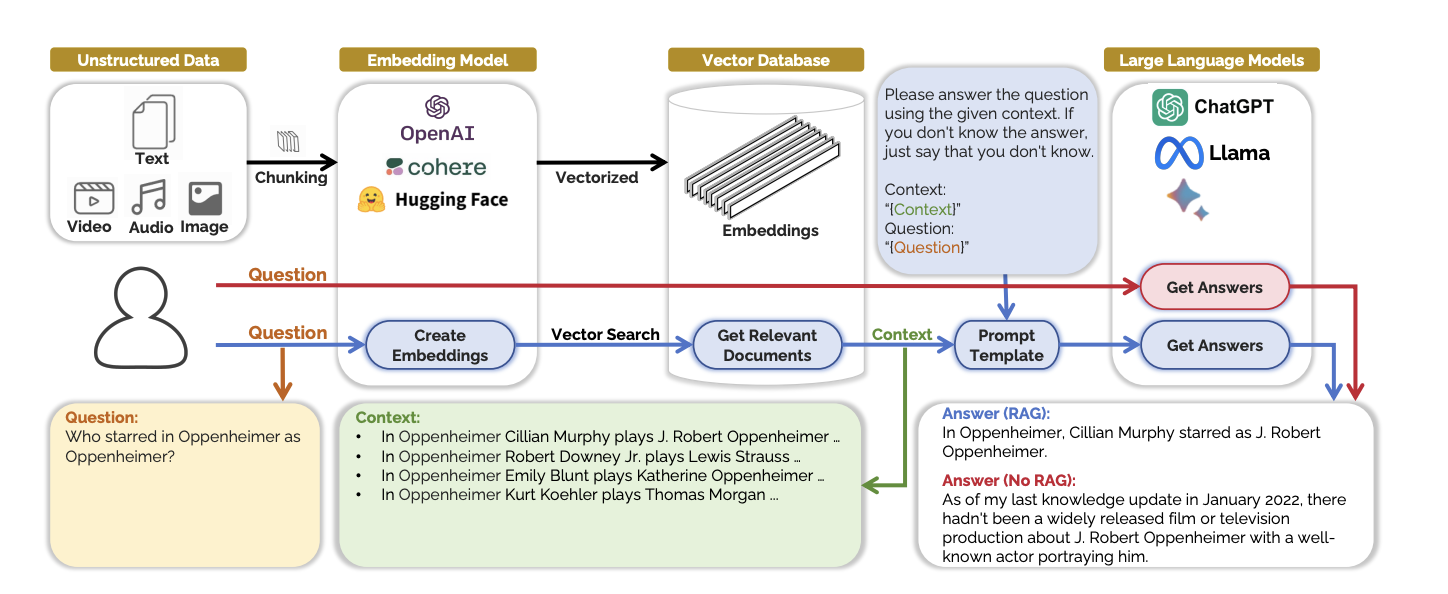
\includegraphics[width=0.85\linewidth]{images/bab-3/embeddings.png}
  \caption{Contoh \emph{RAG framework} yang menggunakan \emph{Vector Database}.}\label{fig:RAG-Framework}\citep{Jing}
\end{figure}

\subsection{Pembuatan Sitasi Otomatis}
Sistem melakukan ekstraksi metadata seperti judul, penulis, tahun, dan DOI dari PDF dan menyusunnya ke dalam format referensi (APA, MLA, IEEE, Harvard) secara otomatis.

\subsection{Anotasi PDF}
Menggunakan integrasi \texttt{PDF.js}, pengguna dapat melakukan:
\begin{itemize}
  \item Highlight teks
  \item Menambahkan catatan
  \item Menyimpan anotasi ke database untuk ditampilkan ulang
\end{itemize}